% !TeX root = ../thuthesis-example.tex

\chapter{集群故障容错和恢复}

\section{基于拓扑感知的查询和写入规划}
上文提到了集群的拓扑感知,总结来说,ConfigNode Leader不但可以探知每一个节点的存活情况,还能够探测DataNode之间的每一个连接。当发现出现网络分区和节点宕机等情况的时候,本文提出的高可用解决办法可以通过对查询和写入规划的改写和三级重试来做到最大限度的错误避免和自动容错,从而保证用户的请求依然能够完成。本节主要介绍基于拓扑感知的查询流程。

\subsection{写入和查询流程概述}

\begin{figure}
  \centering
  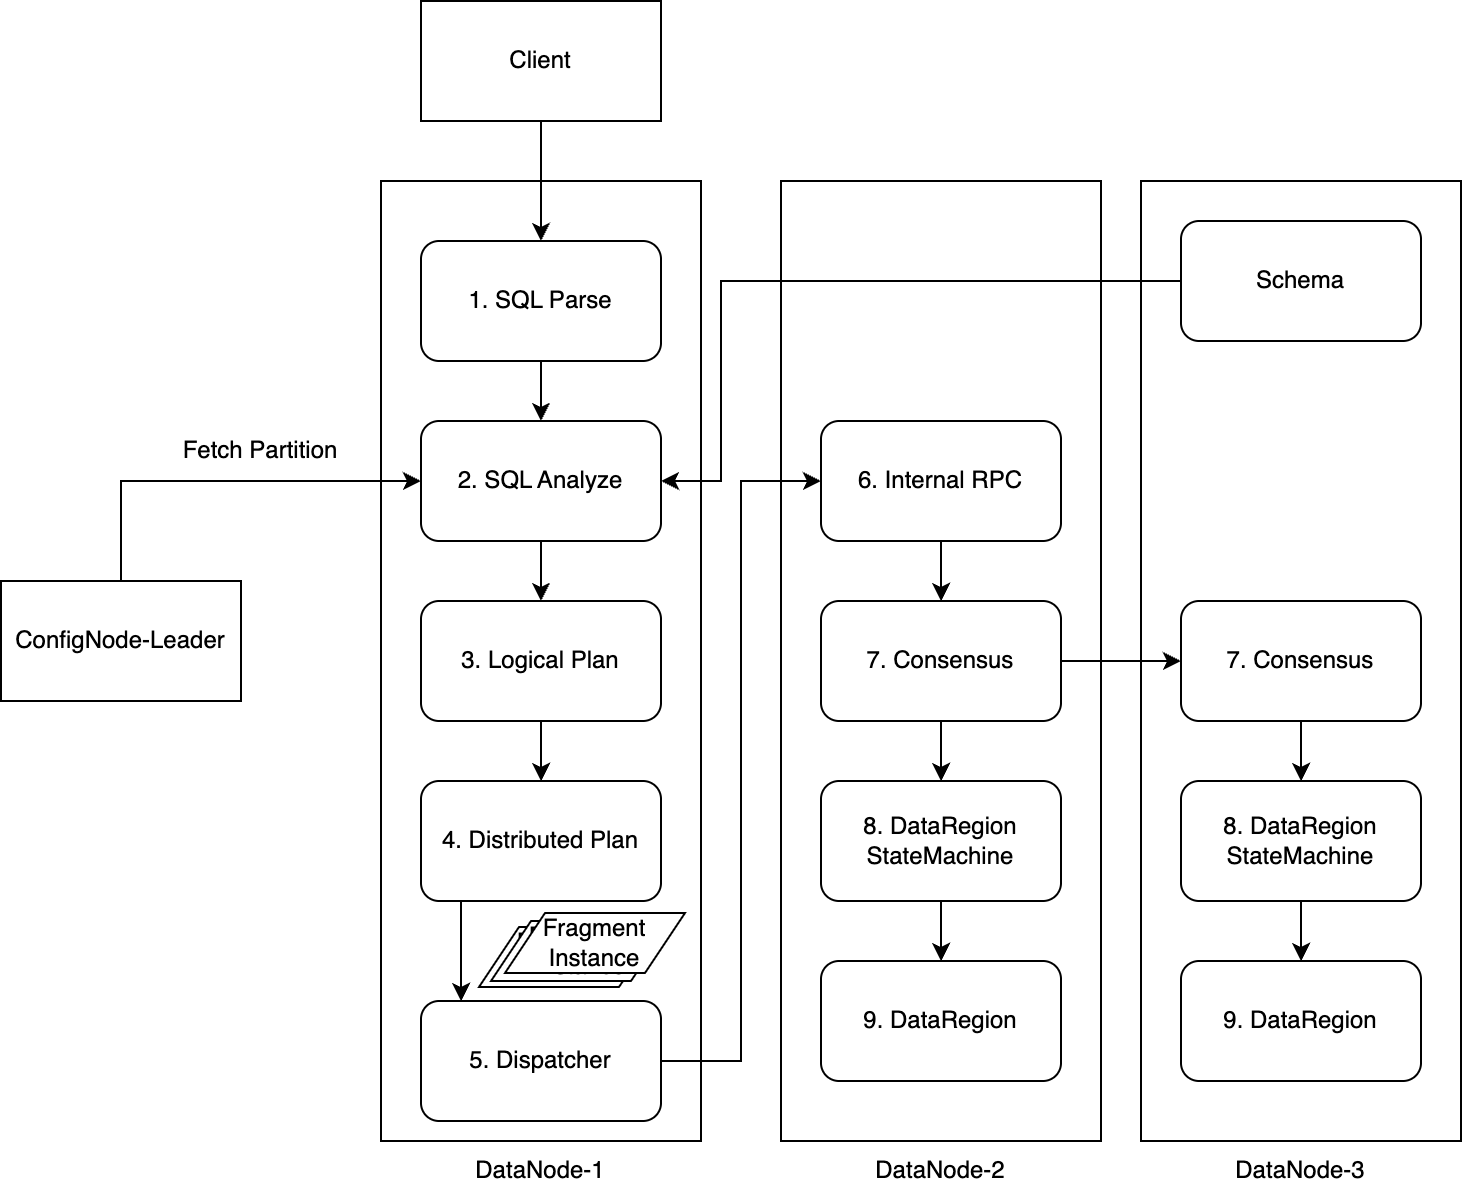
\includegraphics[width=0.99\linewidth]{c04-write-process.png}
  \caption{IoTDB写入全流程}
  \label{fig:c04-write-process}
\end{figure}

图\ref{fig:c04-write-process}展示了IoTDB现有的写入和查询流程。

首先,客户通过SQL等方式请求IoTDB的DataNode,从而发起写入或查询流程。目前,IoTDB集群中的所有DataNode都能对外提供同质化的写入和查询服务,客户端可以选择连接在任意一个DataNode上发出写入的请求。

当客户端的SQL请求到达IoTDB的DataNode之后,第一步会首先对客户端发送的SQL进行解析(SQL Parse)。这一步主要会对SQL进行语法和格式的校验等。

接下来第二步会进入分析阶段(Analyze),本阶段主要准备本次写入或查询执行所需要的数据,主要包含两部分:元数据和集群Region的分区数据。DataNode可能会从ConfigNode这里请求所需要的最新的分区情况,并从其他的DataNode上拉取所需要的元信息。在此步骤上还会校验相关的数据。

在所有的信息都准备到位之后,第三步会进行逻辑计划的生成(Logical Planning)。逻辑计划描述了查询的逻辑操作,但不涉及具体的物理执行细节。逻辑计划通常以树形结构表示,称为逻辑查询树,树的每个节点代表一个逻辑操作符,例如选择、投影、连接、聚合等,树的边表示数据的流动。

有了逻辑计划之后,第四步会进行分布式执行计划的生成(Distributed Planning)。分布式计划是在逻辑计划的基础上,考虑集群数据分布和并行执行的计划方案,它描述了如何在分布式环境中执行查询,包括数据如何在节点上传输、没有依赖的操作可以在哪些节点上并行执行等。
分布式计划的基本组成单元是碎片实例(FragmentInstance)。它代表了分布式执行计划中针对某一个分区Region的操作。每一个FragmentInstance能够保证在一个分区执行内完成,不涉及跨分区的数据搬运。

产生了分布式执行计划之后,第五步就是由调度器去实际调度和执行分布式计划的每一个碎片实例。根据写入或者查询规划的不同,调度器可能将碎片实例调度到本地直接执行,也可能将实例调度到远端执行。如果调度失败,调度器还可能会重试调度。

在理想情况下,每一个实例最终会被交付给共识层进行执行。共识层会进行相关的读写操作的执行,并且提供数据复制和一致性的保证。以Raft共识协议为例,交给共识层的写入操作会保证被复制给大多数节点执行完成之后才会返回成功写入,交给共识层的读取操作能够保证读到线性一致性的结果。

真正执行操作的是IoTDB的单机存储引擎,采用LSM架构\cite{o1996lsmtree},使用MemTable作为内存结构,使用TsFile\cite{zhao2024apachetsfile}作为持久性外部存储。

\subsection{基于拓扑感知的写入流程优化}

在2.0.2.1版本之前,对于需要调度器在远端调度的写入碎片实例,如果写入失败,调度器会进行多次重试,直到达到客户端配置的请求超时时间之后才会返回客户端失败。在网络分区的情况下,客户端的请求可能需要在很长时间的重试之后依然失败。如果在客户端侧没有配置重试的策略,那么这就将会导致这种情况下的客户端数据丢失,RPO不为0的情况。

在拓扑感知的情况下,我们采用了立马失败的策略。当我们检测到网络分区判断出本次执行必将失败的时候,我们会直接在调度之前就失败。

\begin{figure}
  \centering
  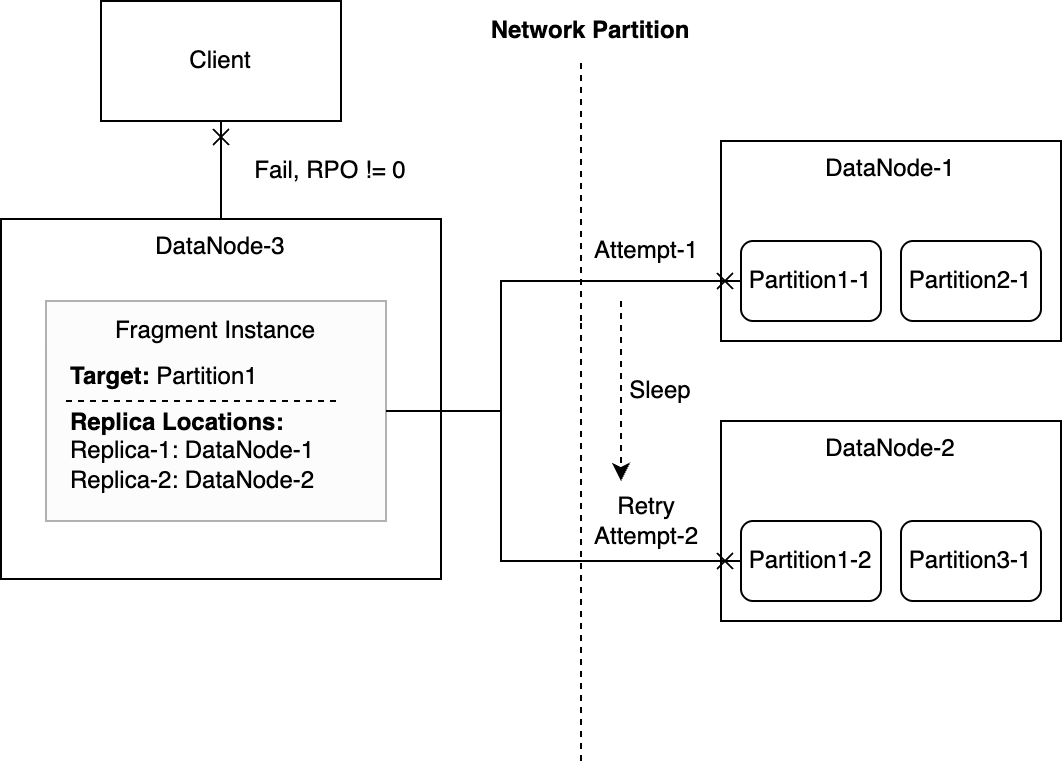
\includegraphics[width=0.9\linewidth]{c04-write-with-topology.png}
  \caption{网络分区下的写入失败情况}
  \label{fig:c04-write-with-topology}
\end{figure}

在\ref{fig:c04-write-with-topology}图中我们可以看到分区的问题。
在IoTDB的集群中,DataNode3和其他两个节点产生了对称分区问题。此时,如果Client连接上了DataNode3执行写入计划,写入计划最终会被解析为FragmentInstance,对象是Partition1。但是不巧的是,Partition1的两个副本分别在DataNode1和DataNode2上,这导致了这个FragmentInstance需要被调度到这两个节点上执行。
在2.0.2.1方案之前,调度器会先尝试调度到DataNode1上,但是由于网络分区的问题,本次请求最终会以超时失败。接着,调度器会尝试选择第二个副本执行,再次尝试调度,但本次请求最终依然会因为分区而失败告终。调度器会反复重复上述的重试策略,直到本次的执行超过客户端指定的超时时间,最终返回客户端失败。

这种写入计划和执行存在两个问题。首先,对于客户端来说,网络分区的错误需要经历一个完整的超时周期(默认配置是1分钟)才会返回,这会严重影响客户端的吞吐。其次,如果客户端不尝试连接其他的DataNode进行重试,那么本次写入失败最终会导致这部分的数据未能被持久化。


在具备拓扑感知功能后,我们可以在规划阶段就解决这个问题。

详细来说,在生成FragmentInstance之后,我们可以提前根据从ConfigNode Leader下发的集群最新拓扑结构对这个FragemntInstance涉及的Partition的所有地点进行可达性计算。如果有些副本所在的节点因为分区等原因不可达,那么就会标记这些副本,在调度的时候避开这些位置。
如果一个FragmentInstance的所有副本位置都不可达,那么调度器就不会调度,而是直接返回客户端这个FragmentInstance写入失败。客户端此时可以配置重试策略,将本次写入请求连接到DataNode-1或者DataNode-2上进行执行,最终实现写入。
总结来说,在具备拓扑感知能力之后,写入请求不会进行长时间的重试,能够立马发回客户端重试。同时,返回时会带上建议的重试节点,帮助客户端完成最后的写入。

\subsection{基于拓扑感知的查询流程优化}

\begin{figure}
  \centering
  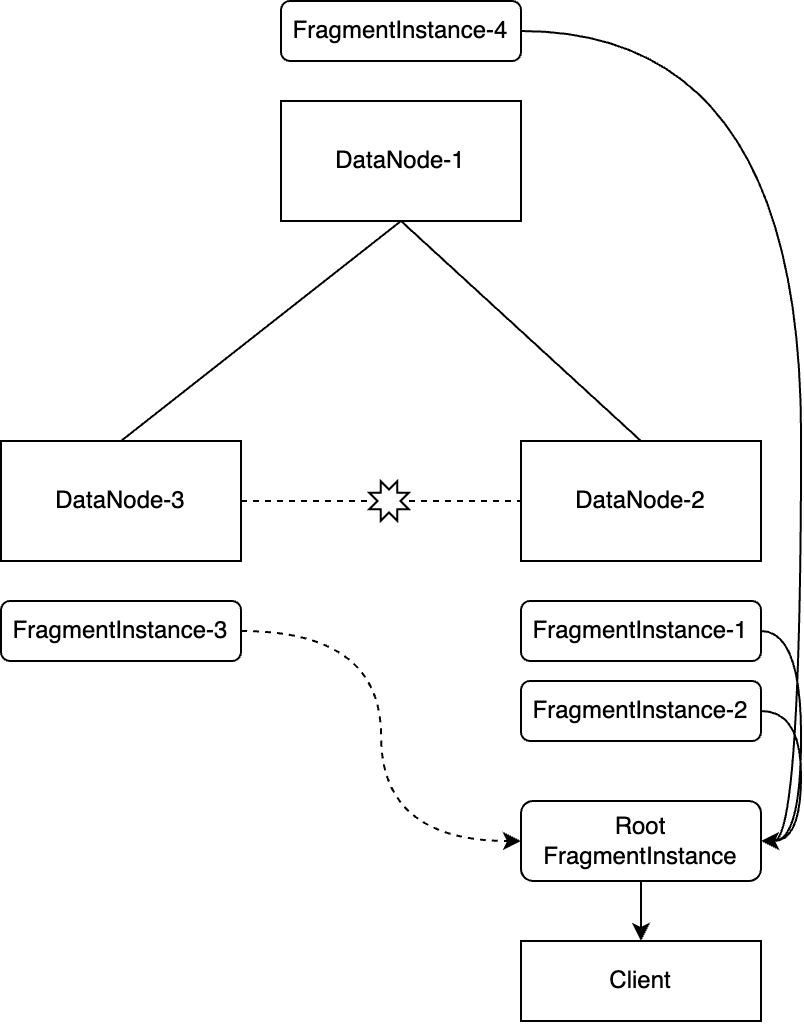
\includegraphics[width=0.7\linewidth]{c04-fi-topology-partition.png}
  \caption{网络分区下的查询失败情况}
  \label{fig:fi-topology-partition}
\end{figure}

在非对称网络分区的情况下,例如图\ref{fig:fi-topology-partition}所示,没有拓扑感知的查询规划可能会导致在资源允许的条件下依然查询失败的错误。在分布式查询计划中,root fragment instance是位于查询计划的顶端的节点,负责最终结果的聚合,需要收集其他碎片实例的结果,也是最终返回结果的那个计算节点。

例如图中所示,本次查询计划涉及4个FragmentInstance,分别会被调度到DataNode的1,2,3节点上实现。本次查询的root instance 被调度到了DataNode2上,出于最小化数据在节点之间传输的考虑。在DataNode2和DataNode3之间发生非对称网络分区的时候,DataNode-2上的root Fragemtn Instance并不能成功连接DataNode3并且拉取对应的数据,这导致了本次查询的失败。

在有了拓扑感知算法之后,本次查询规划的时候可以把root FragmentInstance调度到DataNode1节点上,这样即使在出现了非对称网络分区的情况下,DataNode1依然可以连接到剩下的两个节点,位于DataNode1上的root FragmentInstance可以成功拉取本次查询规划的所有的instance的数据。

再次我们给出基于网络拓扑分区的root fragment instance的算法描述。
\begin{algorithm}
  \caption{查找DataNode和FragmentInstance候选}
  \label{alg:find_candidates}
  \begin{algorithmic}
  \REQUIRE 集群拓扑结构 (连通图), FragmentInstance列表
  \ENSURE DataNode候选列表, FragmentInstance候选列表
  
  \STATE $DataNodeCandidates \leftarrow \emptyset$
  \STATE $FragmentInstanceCandidates \leftarrow \emptyset$
  
  \FOR{每个 DataNode $node$ 在 集群拓扑结构 中}
      \STATE $isCandidate \leftarrow true$
      \FOR{每个 FragmentInstance $instance$ 在 FragmentInstance列表 中}
          \STATE $foundConnection \leftarrow false$
          \FOR{每个 Replica $replica$ 在 $instance.ReplicaSet$ 中}
              \IF{$node$ 和 $replica$ 在 连通图 中连通}
                  \STATE $foundConnection \leftarrow true$
                  \STATE \textbf{break} \COMMENT{找到一个连接即可}
              \ENDIF
          \ENDFOR
          \IF{$foundConnection = false$}
              \STATE $isCandidate \leftarrow false$
              \STATE \textbf{break} \COMMENT{如果和任何ReplicaSet都无法连通,则不是候选}
          \ENDIF
      \ENDFOR
      \IF{$isCandidate = true$}
          \STATE $DataNodeCandidates \leftarrow DataNodeCandidates \cup \{node\}$
      \ENDIF
  \ENDFOR
  
  \FOR{每个 FragmentInstance $instance$ 在 FragmentInstance列表 中}
      \STATE $isCandidate \leftarrow false$
      \FOR{每个 DataNode $candidate$ 在 $DataNodeCandidates$ 中}
          \FOR{每个 Replica $replica$ 在 $instance.ReplicaSet$ 中}
              \IF{$candidate = replica$}
                  \STATE $isCandidate \leftarrow true$
                  \STATE \textbf{break} \COMMENT{找到一个候选DataNode即可}
              \ENDIF
          \ENDFOR
          \IF{$isCandidate = true$}
              \STATE \textbf{break} \COMMENT{找到一个候选DataNode即可}
          \ENDIF
      \ENDFOR
      \IF{$isCandidate = true$}
          \STATE $FragmentInstanceCandidates \leftarrow FragmentInstanceCandidates \cup \{instance\}$
      \ENDIF
  \ENDFOR
  
  \RETURN $DataNodeCandidates$, $FragmentInstanceCandidates$
  \end{algorithmic}
  \end{algorithm}

\section{错误时期的三级重试和Failover}

为了确保系统在面临各种故障时仍能保持高可用性和数据一致性,我们采用了一种基于重试的故障转移策略。具体而言,我们设计了一种三级重试机制,该机制涵盖了客户端、协调者以及共识层。通过在这些关键层面上实施重试,我们旨在最大程度地提高错误恢复的成功率,确保即使在不利条件下,系统也能正确处理并解决问题。这种多层次的重试策略不仅增强了系统的鲁棒性,还显著提升了其在复杂分布式环境中的可靠性。

整个三级重试的的实现方案。

\subsection{Session的重定向重试}

在Apache IoTDB中,Session扮演着至关重要的角色,它不仅是客户端应用程序与IoTDB DataNode集群之间进行通信的桥梁,更是实现服务自动发现的关键组件。具体来说,Session封装了与IoTDB服务器建立连接、发送请求、接收响应等一系列底层操作,为应用程序提供了简洁高效的API接口。通过Session,客户端能够轻松地执行数据写入、查询、元数据操作等任务,而无需关心复杂的网络通信细节。此外,Session还具备自动发现DataNode集群服务的能力,这意味着即使集群拓扑结构发生变化,客户端也能自动适应并保持与可用节点的连接,从而确保了系统的高可用性和稳定性。值得注意的是,Session的设计充分考虑了性能和安全性,它通过连接池等机制来减少连接建立的开销,并通过身份验证和权限控制等手段来保障数据的安全性。因此,Session是IoTDB客户端应用程序开发中不可或缺的核心组件。

Session侧的重试是高可用的重要组成部分,是DataNode服务发现和负载均衡的基础。通常来讲,客户端依赖Session连接到集群中的某一个特定DataNode上执行相关的操作请求。然而,如果该DataNode节点突发故障,例如进程宕机、因网络分区而导致连接中断、高负载状态下导致资源耗尽而不能很好地提供服务,此时Session就能通过执行超时和连接通道来检测出异常的发生,并启动故障转移的流程,将请求自动连接到其他的节点中完成。
通过这种无缝切换,Session不但保证了客户端的请求能够被路由到健康的节点上执行,从而保证了数据写入操作的正确性和可靠性,也同样实现了负载均衡的能力。

每一个Session启动的时候,都会配置至少一个DataNode节点和ConfigNode的节点。在Session创建之后,会启动一个后台的进程,这个进程会从集群的大脑ConfigNode中定期拉取所有DataNode的列表和其对应的状态。当当前的DataNode出现问题的时候,Session就会根据列表的顺序不断尝试下一个可用的DataNode。这种实现方式还有一个额外的好处。当集群增加一个新的DataNode的时候,不需要对现在存活的Session进行修改配置并且启动,这个机制能够自动让现有的Session发现这些新增的DataNode,并将数据引导到新的DataNode上。

DataNode在写入的时候,还会进行Redirect的提示,这个行为是集群自动负载均衡的重要能力之一。Session在初始创建的时候,可以默认连接到任何一个DataNode上。当DataNode处理完了这个连接的请求的时候,会根据集群的综合情况考虑,在返回结果的地方增加一个建议重定向的字段,该字段的用意是希望Session后续的连接能够重定向到其他节点上来执行。在处理带有重定向标志的Session的时候,Session会将底层的连接信道重新导引到那个新的DataNode之上,通常,当需要读写的副本的leader节点所在DataNode的时候,才会发生这样的重定向导引活动。

此外,在出现了上述提到的非对称网络分区的时候,查询规划和计划也会建议重定向。如上述所言,如果在非对称分区的时候rootInstance没有地方摆放,那么返回给Session的报错信息就会加上重定向的DataNode,这个DataNode往往能够放置这个root instance。


总结来说,Session侧的重试实现了服务发现、自动转移、负载均衡和容错的能力。



\subsection{协调者}

协调者(Coordinator)是IoTDB的重要组成部分,他负责接受客户端的SQL请求,负责SQL解析、物理计划和分布式执行计划的生成,对每一个FragmentInstance进行调度和执行,以及最终结果的的收集和返回。

协调者侧重试的目的是避免因为单副本、单节点的失效而影响查询和写入的能力。通过充分利用底下共识模块提供的多副本的能力,协调者能够在某个副本写入失败的时候自动转移到另外一个副本上,从而规避系统的暂时性错误。






\subsection{Client的重试策略}






\subsection{熔断和降级措施}



